\section{Representing Social World States for Better Social Reasoning}
\label{sec:social_understanding}
We first demonstrate the effectiveness of our \protocolname representations towards social reasoning by evaluating various LLMs across diverse static third-person perspective social reasoning tasks. We explore the following social reasoning question-answering (QA) tasks:


\paragraph{ToMi \& ParaToMi} 
ToMi \citep{Le2019RevisitingTE} is one of the most important benchmarks for evaluating the theory-of-mind abilities of models.
Inspired by the Sally-Anne test, the ToMi dataset evaluates whether models can infer an agent's belief about an object's location after a sequence of actions by multiple agents, which may or may not move the object. 
\textbf{ParaToMi} \citepcustom{\textbf{Para};}{sclar2023mindinglanguagemodelslack} is a revised version of ToMi \citep{Le2019RevisitingTE} that addresses the limited linguistic diversity of the original by rewording all templates. The resulting dataset is more complex, as actions are expressed in a less straightforward way. 
For both ToMi and ParaToMi, we randomly sample 600 questions from the dataset.
We measure accuracy by whether the model correctly infers the agent's belief about the object's location.

\paragraph{HiToM} \citep{wu-etal-2023-hi} evaluates higher-order theory of mind (ToM) in LLMs, requiring recursive reasoning about others’ beliefs. It extends ToMi by adding agent interactions—such as chatting, deception, and joint attention—beyond simple object movement. The task concludes with a belief inference question about an object’s location. We randomly sample 72 scenarios (100 questions total) and report accuracy based on the model’s ability to infer the correct agent belief.

\paragraph{FANToM} \citepcustom{\textbf{FAN};}{kim-etal-2023-fantom} is a multi-party conversation question-answering dataset designed to test coherent theory-of-mind capabilities. 
In FANToM, speakers join and leave the conversation while it continues, making participants hold both false and true beliefs. The benchmark includes first-order and second-order theory-of-mind questions about the beliefs of conversation participants. We use 64 sampled conversations from the short version of FANToM, containing a total of 1,086 questions. We report \texttt{All Qs} metric, requiring the model to correctly answer all questions for a given conversation snippet.

\paragraph{MMToM-QA} \citepcustom{\textbf{MMToM;}}{jin-etal-2024-mmtom} is multi-modal question-answering benchmark for theory of mind reasoning, focused on jointly inferring goals and beliefs in everyday object search scenarios. We use the text-only subset (describing search behavior) and evaluate on 300 randomly sampled, balanced questions covering belief (true/false, short/long-term) and goal inference (true/false beliefs, updates, future actions).

\begin{table}[ht!]
    \centering
    \small
    \caption{Performance comparison of models with CoT and with \protocolname representations (generated by O3) on various social reasoning tasks. Bolded values indicate the best average performance across models. \update{%
    L4 means Llama 4, 4o means GPT-4o, o3m means o3-mini.}
    } 
    
    \begin{tabular}{lccccc}
        \toprule
        \textbf{Model} & \textbf{ToMi} & \textbf{Para} & \textbf{HiToM} & \textbf{FAN} & \textbf{MMToM} \\
        \midrule
        \texttt{L4} \tiny{\textit{CoT}} & 0.655 & 0.740 & 0.720 & 0.264 & 0.443 \\
        \texttt{L4} \tiny{\textit{\protocolname}} & 0.662 & 0.763 & 0.700 & 0.415 & 0.450 \\
        \midrule
        \texttt{4o} \tiny{\textit{CoT}} & 0.813 & 0.818 & 0.660 & 0.396 & 0.652 \\
        \texttt{4o} \tiny{\textit{\protocolname}} & 0.927 & 0.905 & 0.750 & 0.491 & 0.692 \\
        \midrule
        \texttt{o3m} \tiny{\textit{CoT}} & 0.863 & 0.817 & 0.810 & 0.057 & 0.493 \\
        \texttt{o3m} \tiny{\textit{\protocolname}} & 0.960 & 0.900 & 0.860 & 0.170 & 0.506 \\
        \midrule
        \texttt{R1} \tiny{\textit{CoT}} & 0.945 & 0.893 & 0.420 & 0.491 & 0.374 \\
        \texttt{R1} \tiny{\textit{\protocolname}} & 0.980 & \textbf{0.950} & 0.510 & 0.547 & 0.437 \\
        \midrule
        \texttt{o1} \tiny{\textit{CoT}} & 0.952 & 0.835 & 0.870 & 0.415 & 0.725 \\
        \texttt{o1} \tiny{\textit{\protocolname}} & \textbf{0.985} & 0.932 & \textbf{0.880} & \textbf{0.623} & \textbf{0.785} \\
        \bottomrule
    \end{tabular}
    \label{tab:social_reasoning}
\vspace{-2em}
\end{table}



\subsection{Experimental Setup}
\label{sec:experimental_setup}
We use off-the-shelf LLMs to parse narratives into \protocolname representations in the JSON format for ease of computation (parser model). Unlike other ToM methods \citep{sclar2023mindinglanguagemodelslack}, our representation is general and task-agnostic as we use the same parser prompt across all benchmarks, with minimal adjustments only when benchmarks impose artificial constraints (e.g., ToMi's assumption that characters automatically know all object locations upon entering a room). Importantly, \protocolname parsing is query-independent, creating a general-purpose social world representation for the same narrative without access to downstream questions.

For downstream reasoning tasks, we concatenate the original narrative with its \protocolname representation and ask the LLM to answer the question (QA model).
Our evaluation spans five state-of-the-art LLMs: \texttt{GPT-4o}, \texttt{o1}, \texttt{o3-mini}, Deepseek-R1 (\texttt{R1}), and Llama 4 Maverick Instruct (\texttt{Llama 4}).
Note that we ensure a fair comparison by enforcing that \protocolname uses identical source information (i.e., the same narrative) as baselines while providing structured social world representations.
We use the Chain-of-Thought (CoT) method as the baseline across all tasks and models (See a more comprehensive baseline comparison in \S \ref{sec:efficiency_analysis}).
To maximize reproducibility, we use temperature 0.0 for all models.

\subsection{Main Results Across Tasks and Models}
\label{sec:omniscient_social_reasoning}


Table~\ref{tab:social_reasoning} shows \protocolname consistently outperforms the CoT baseline across all evaluated tasks when averaged across models (e.g., from 0.84 to 0.90 on ParaToMi) \footnote{We use O3 as the parser model here for consistency. Additional experiments with different parsing models show consistent trends (Appendix \ref{app:add_results}).}. The improvements are especially pronounced in benchmarks requiring complex social reasoning. For instance, FANToM, a benchmark with long, complex multi-agent dialogues, sees the largest average boost of +11.1 points (from 0.39 to 0.50).
Surprisingly, even smaller models such as \texttt{o3-mini} and Llama 4 benefit substantially. \texttt{o3-mini} improves on ToMi from 0.86 to 0.96, and Llama 4 shows an increase on FANToM from 0.26 to 0.42. These gains suggest that \protocolname helps models disambiguate agent perspectives and maintain coherent mental state tracking even with limited capacity.

To better isolate and understand the effectiveness of the \protocolname representations, rather than effects driven by memorization or training contamination, we use ParaToMi for the following ablation studies. ParaToMi requires an access code to obtain, it is less likely to have been included in the training data of most LLMs.
\begin{figure}[t]
\centering
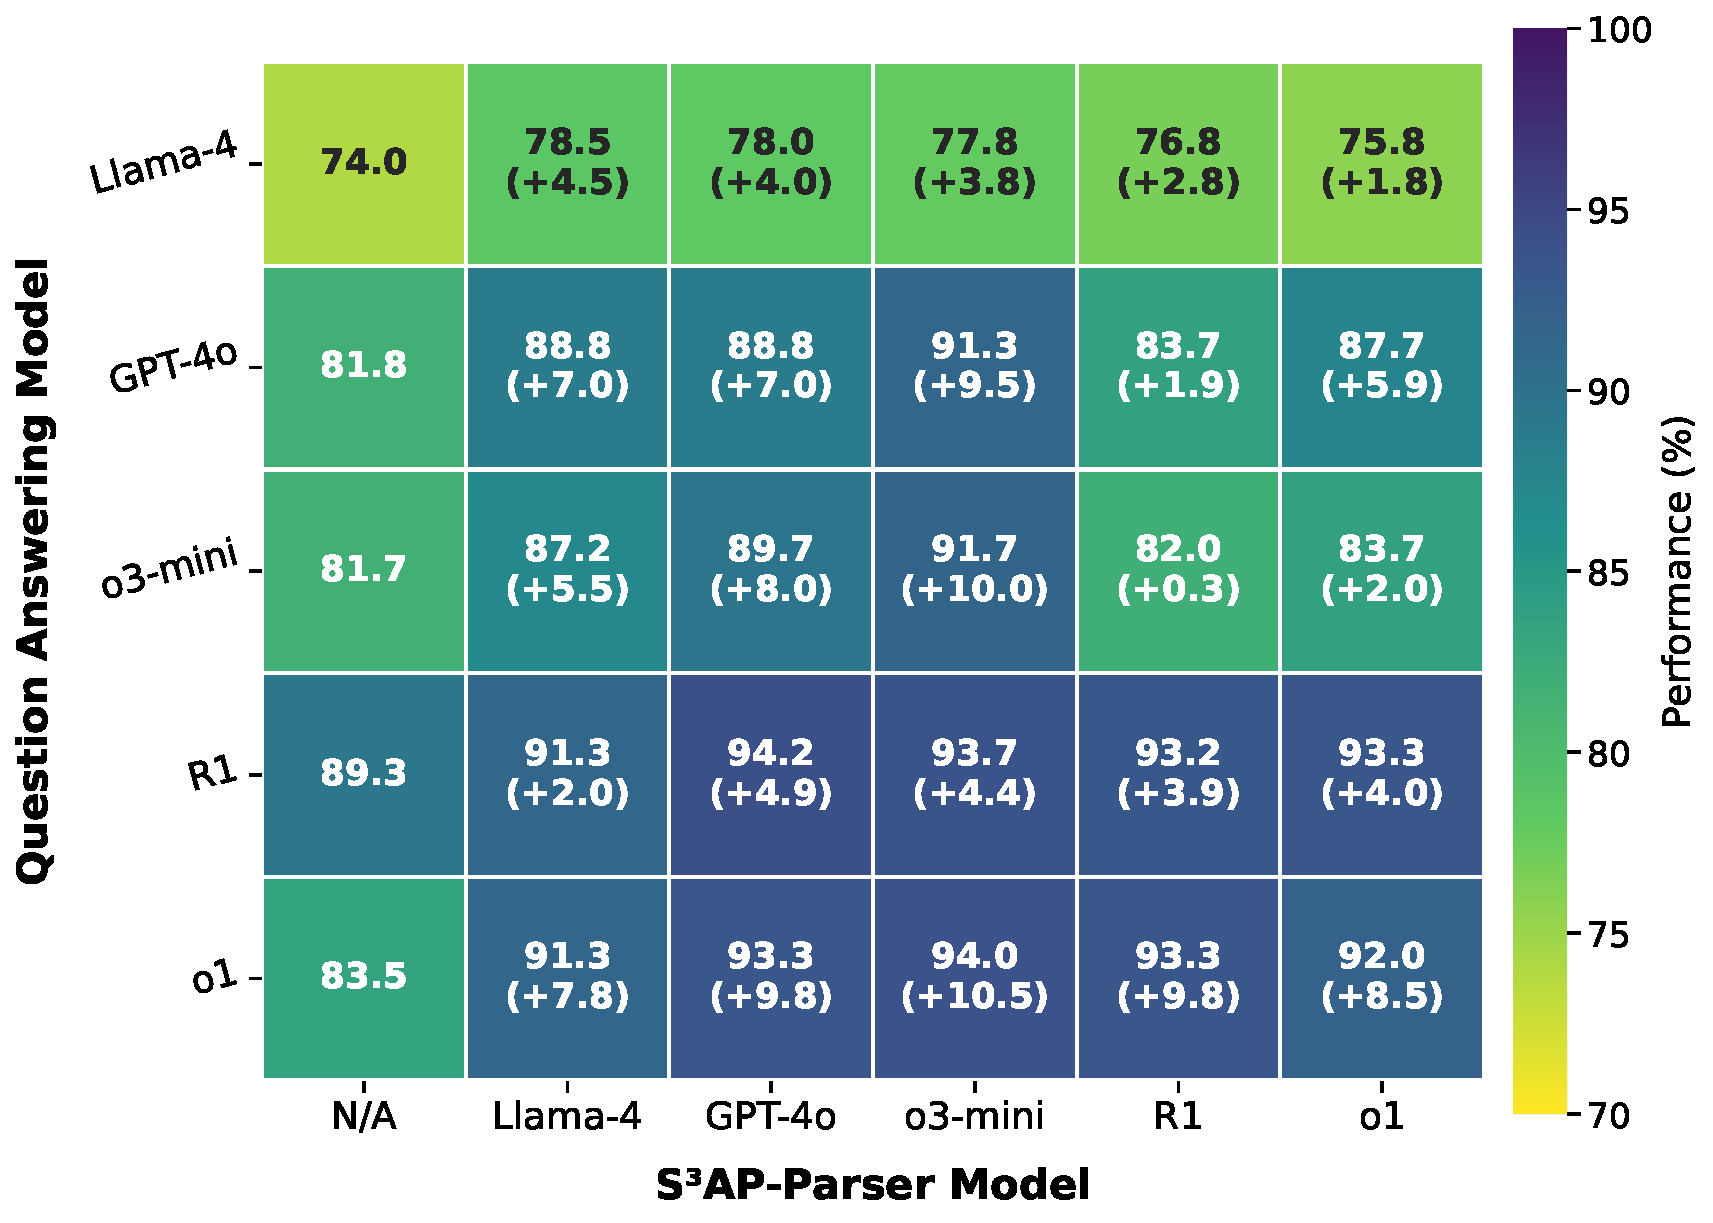
\includegraphics[width=\linewidth]{figs/model_relative_gain_heatmap.pdf}
\caption{Performance of different models on ParaToMi using \protocolname representations generated by various models. Numbers in parentheses show performance change.}
\label{fig:protocolname_quality_correlation}
\end{figure}


\paragraph{Effect of the parser model}
To investigate how the abilities of the parser model affect reasoning, we use different models to generate \protocolname representations and apply them to various models for the ParaToMi task.
Surprisingly, we find that models generally benefit from the \protocolname representations generated by a wide range of LLMs, \textit{regardless} of the LLMs' own performance in the social reasoning tasks (Figure~\ref{fig:protocolname_quality_correlation}).
For example, despite \texttt{o3-mini}'s 82\% lower accuracy on the ParaToMi task, it can generate \protocolname representations that boost the \texttt{o1} model's accuracy from 84\% to 94\%.
This finding suggests that so-called ``social reasoning'' may involve two distinct but related components: (1) the ability to track and construct representations of the social world, and (2) the ability to use such representations to answer questions about the mental states of other agents. 
Importantly, a model's weak performance on social reasoning tasks does not necessarily imply deficiencies in the social representation construction. 
This two-part view is consistent with insights from research focusing on the physical world models \citep{worldmodels2018david, LeCun2022, yerukola2024pope}.

\paragraph{Influence of the size of the QA model}
\update{To understand how QA models with various sizes and reasoning abilities benefit from well-formed \protocolname representations (generated by O3), we also conducted experiments on the Qwen3 suite (ParaToMi task; 100 randomly sampled instances), ranging from 0.6B to 80B parameters. S³AP consistently outperforms CoT across all scales.
As shown in Table~\ref{tab:qwen_effect}, \protocolname provides gains even for smaller QA models, while providing larger performance gains for larger models.}


\begin{table}[t]
    \centering
    \small
    \caption{ParaToMi accuracy (\%) with CoT vs \protocolname on Qwen3 models. $\Delta$ (pp) stands for the absolute performance difference .}
    \label{tab:qwen_effect}
    \begin{tabular}{lccc}
        \toprule
        \textbf{Model} & \textbf{CoT} & \textbf{S³AP} & \textbf{$\Delta$ (pp)} \\
        \midrule
        Qwen3-80B   & 77 & 91 & +14 \\
        Qwen3-32B   & 75 & 88 & +13 \\
        Qwen3-7B    & 44 & 45 &  +1 \\
        Qwen3-0.6B  & 48 & 50 &  +2 \\
        \bottomrule
    \end{tabular}
\end{table}



\begin{figure}[t]
\centering
\fbox{\begin{minipage}{0.95\columnwidth}
\small
\textbf{Illustrative Example of Social Context Parsing Failure}

\textit{Scenario:} Evelyn places persimmon in basket $\to$ 
Amelia visits garden $\to$ Amelia leaves $\to$ 
Evelyn moves persimmon to bucket

\textit{Question:} Where does Amelia think Evelyn searches for the persimmon?

\textbf{Incorrect parsing:}
\footnotesize
\vspace{0.1em}
\texttt{\{}\\
\texttt{~~"state": "Evelyn moved persimmon to bucket.}\\
\texttt{~~~~~~~~~~~~Amelia is away.",}\\
\texttt{~~"observations": [}\\
\texttt{~~~~"Evelyn: <same\_as\_state />",}\\
\texttt{~~~~"Amelia: <same\_as\_state />" $\leftarrow$ \textbf{WRONG}:}\\
\texttt{~~~~Amelia can't observe events after leaving}\\
\texttt{~~]}\\
\texttt{\}}
\vspace{0.1em}

\small
\textit{Result:} Incorrect parsing leads to wrong prediction 
(\textit{bucket}) instead of correct answer (\textit{basket}).
\end{minipage}}
\caption{Illustrative example of social context parsing failure from error analysis.}
\label{fig:error_analysis}
\end{figure}

\begin{figure}[t]
\centering
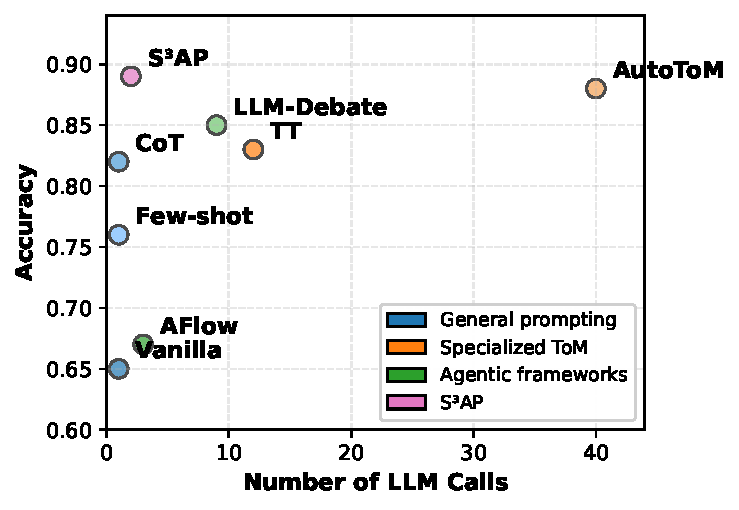
\includegraphics[width=\linewidth]{figs/tom_performance_scatter.pdf}
\caption{Number of LLM calls vs accuracy comparison of ToM methods on ParaToMi with \texttt{GPT-4o} (for both the parser and the QA model). The baselines include specialized ToM methods (TT, AutoToM) and agentic frameworks (AFlow, LLM-Debate). \protocolname achieves the highest accuracy with a low number of LLM calls.}
\label{fig:tom_specialized_baseline}
\end{figure}

\begin{figure}[t]
    \centering
    \begin{minipage}{\columnwidth}
        \small
        \begin{algorithm}[H]
        \begin{algorithmic}[1]
        \STATE \textbf{function} \textsc{ForeseeAndAct}(social world state $s$, agent actions $\mathcal{A}$, goal $g$)
            \STATE $cur\_act \gets \text{SampleAction}(\mathcal{A}, s, g)$
            \STATE $s_{\text{next}} \gets \text{SWM}(s, cur\_act)$
            \STATE $re\_act \gets \text{ActFromSim}(\mathcal{A}, [s_{\text{next}}], s, g)$
            \STATE \textbf{return} $re\_act$
        \STATE \textbf{end function}
        \end{algorithmic}
        \end{algorithm}
    \end{minipage}

    \vspace{1em}
    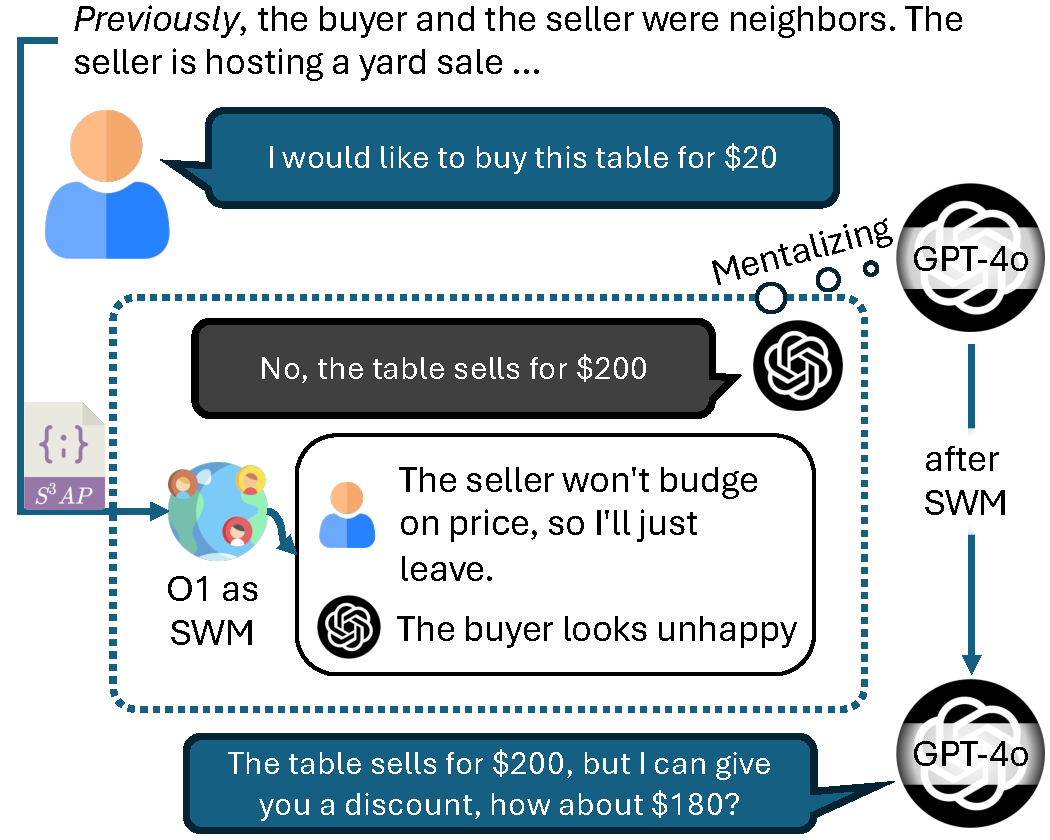
\includegraphics[width=\columnwidth]{figs/swm-agent-fig4.pdf}

    \caption{\texttt{Foresee and Act} with Social World Model (one-step lookahead). The agent uses a social world model to simulate the consequence of a candidate action before committing to a refined action.} %
    \label{fig:swm-agent}
\end{figure}

\begin{figure*}[ht]
    \centering
    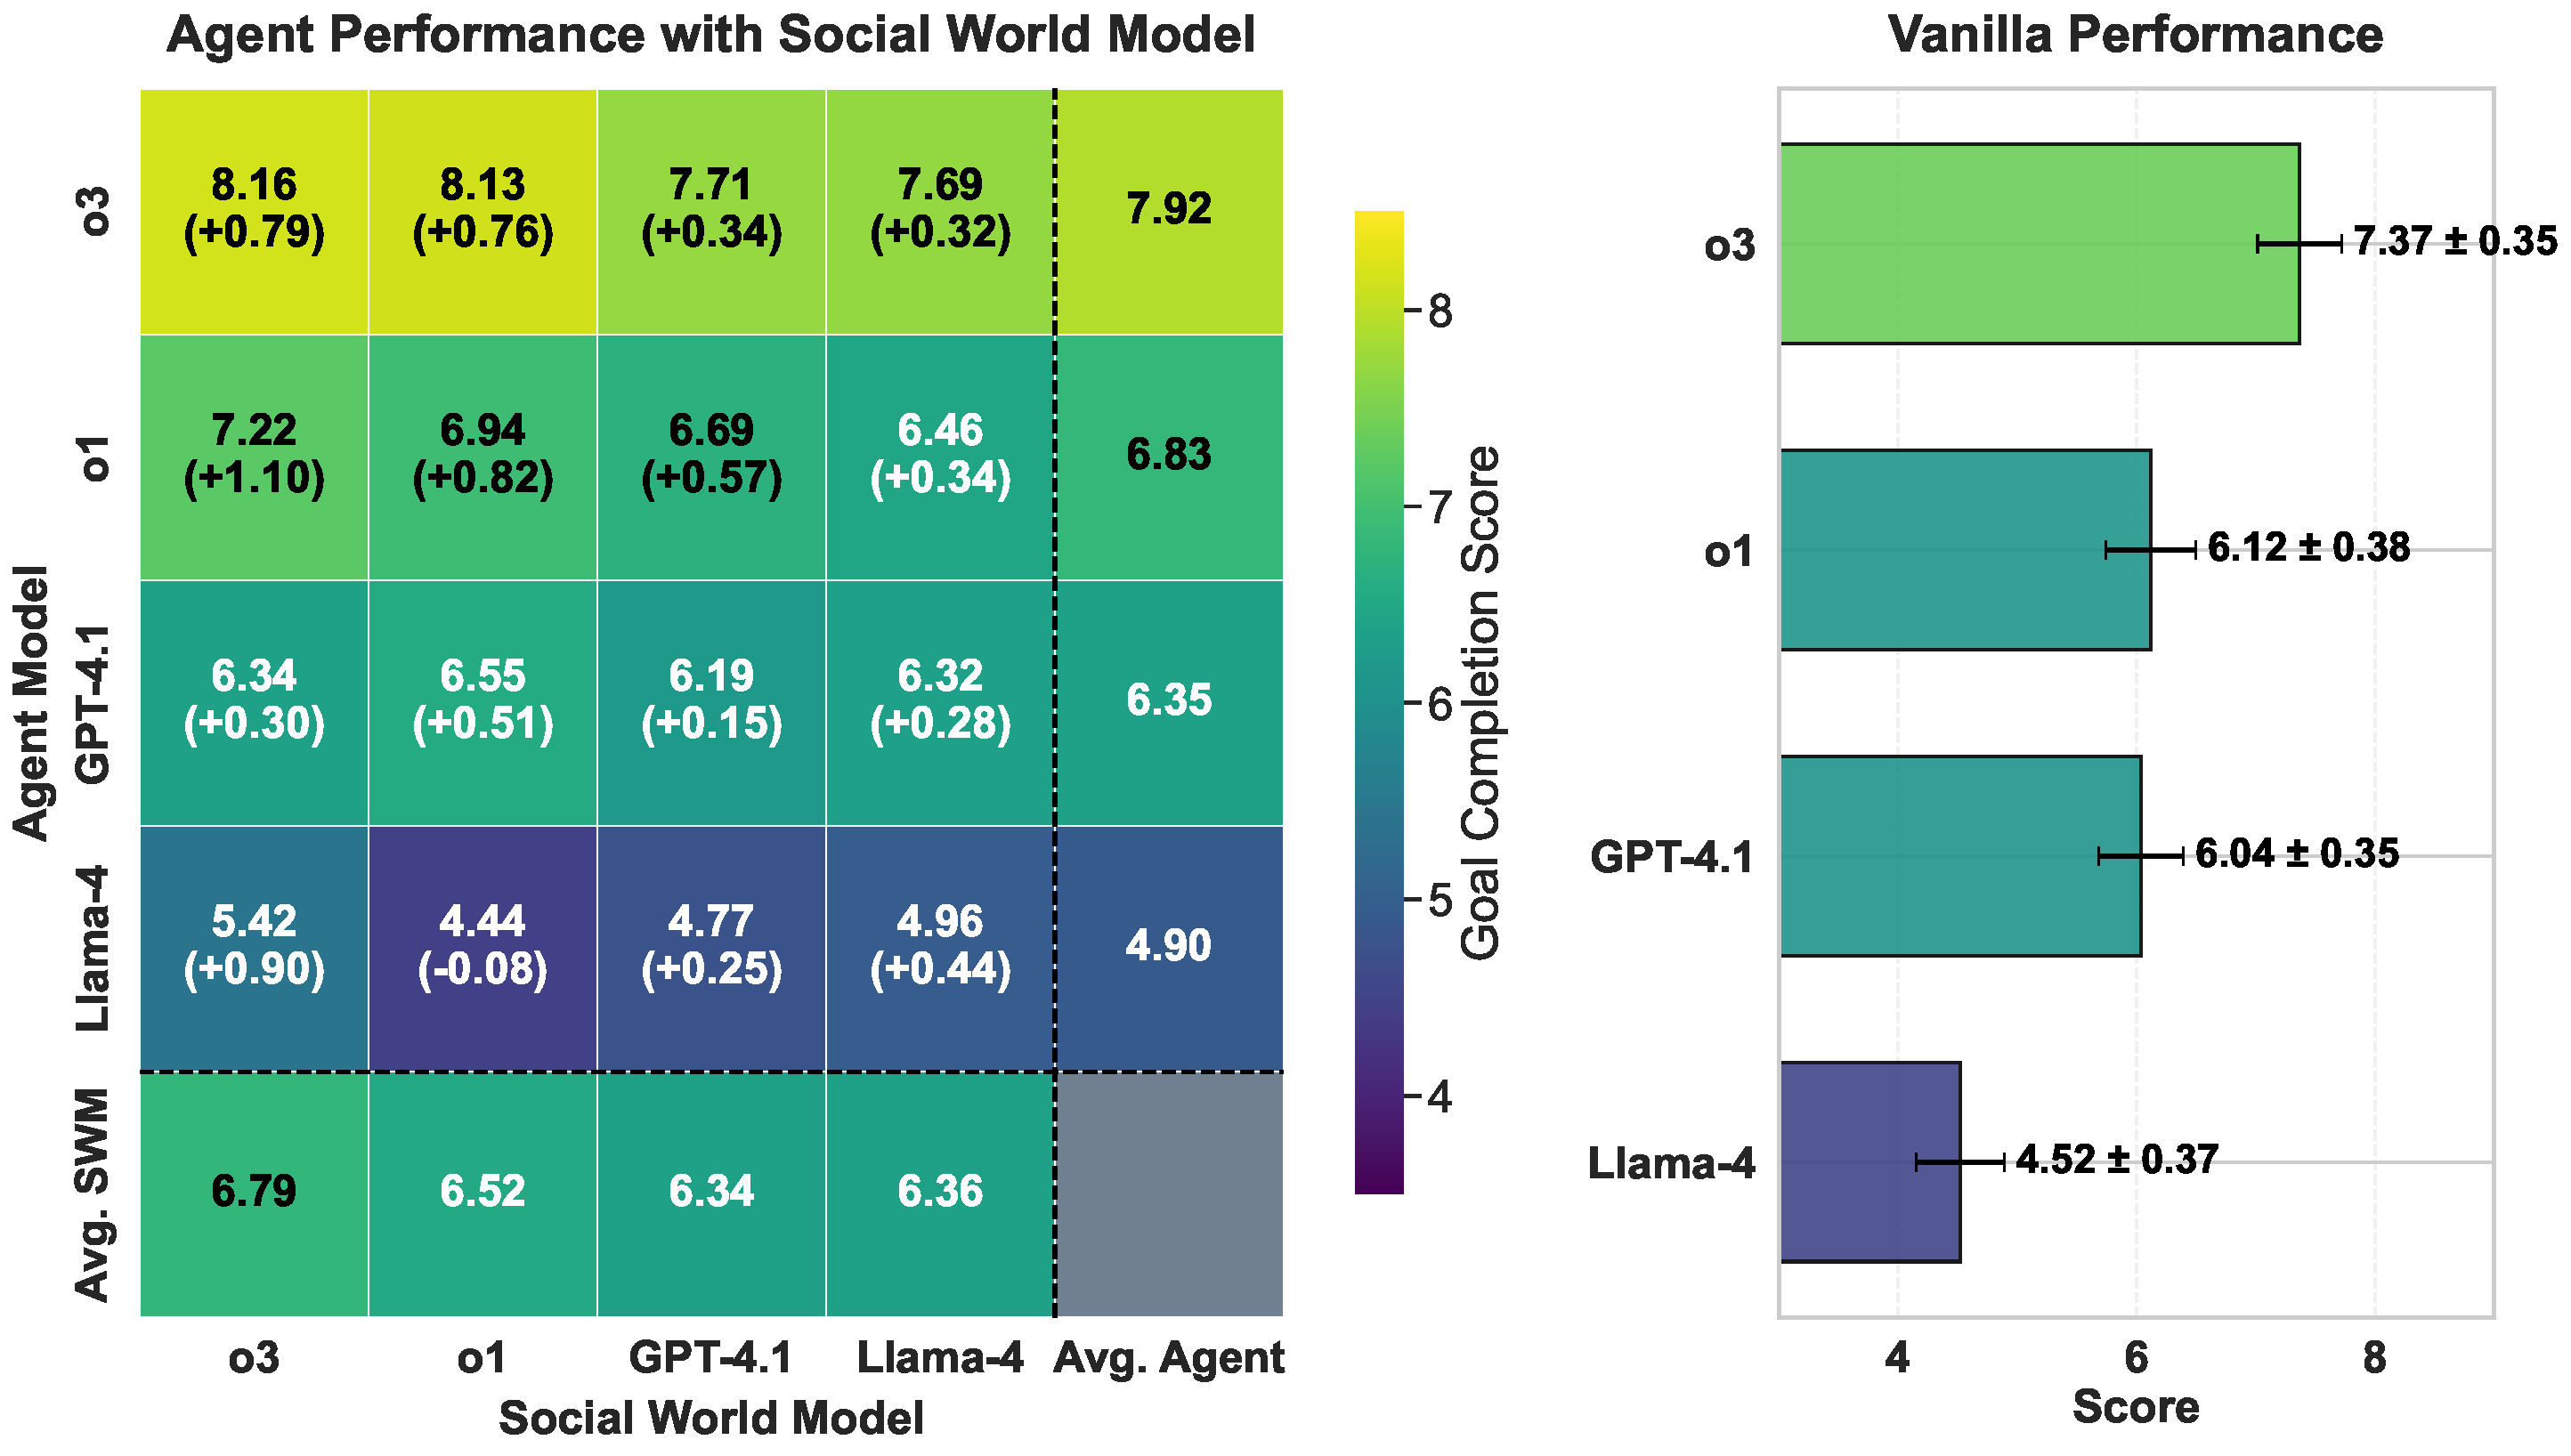
\includegraphics[width=0.85\textwidth]{figs/model_performance_comparison.pdf}
    \caption{Model performance comparison on SOTOPIA-hard eval set. The left panel shows the performance of various LLMs when coupled with different social world models, while the right panel shows baseline performance without a social world model. Values represent goal completion scores (0-10 scale), with higher scores indicating better achievement of social objectives. Numbers in parentheses indicate relative performance change compared to the corresponding baseline.} %
    \label{fig:model_performance_comparison}
\end{figure*}


\paragraph{Parser Quality and Error Analysis}
\update{
To understand the quality of the \protocolname representations generated by different models, and how it affects the downstream performance, 
we first manually created \protocolname representations for 100 scenarios from ParaToMi serving as the ground truth. We then generate \protocolname representations on the same scenarios using various models and evaluated parser quality using an LLM-as-a-judge (GPT-5). Specifically, we asked GPT-5 to rate the quality of the generated \protocolname representation by comparing it to the ground truth \protocolname representations, which eventually outputs a score on a scale of 0 to 1.
While an LLM judge is imperfect, the judge, validated manually, is only used to scale comparisons between a generated parse and the same fixed ground-truth for each instance \footnote{Please refer to Appendix \ref{app:parser_quality} for more details.}.

Interestingly, we find that the parser scores correlate with relative improvement in downstream performance (we average the relative improvement over the CoT baseline across all QA models for each parser model in Figure~\ref{fig:protocolname_quality_correlation}): \texttt{o3-mini} (0.707 score, +7.64\% improvement), \texttt{o1} (0.650, +4.44\%), \texttt{GPT-4o} (0.620, +6.74\%), \texttt{Llama-4} (0.591, +5.36\%), and \texttt{DeepSeek-R1} (0.490, +3.74\%). Notably, smaller models like \texttt{o3-mini} can achieve high parsing scores, suggesting that social parsing capability is distinct from general reasoning ability.

To further understand how the errors in \protocolname representations propagate to the downstream performance, we conducted a detailed analysis of 64 randomly sampled misclassified cases from the ParaToMi benchmark (\texttt{o1} as both the parser and the QA model).
 We find that the vast majority of errors (79.7\%) stem from social context parsing failures (see Figure~\ref{fig:error_analysis}), where models fail to correctly understand and represent the social world state described in the narrative.
The remaining errors are split between pure reasoning failures (7.8\%) and unspecified cases (12.5\%).
These findings suggest that building a successful representation of the social world state is the key for successful social reasoning.}



\subsection{Comprehensive Baseline Comparison}
\label{sec:efficiency_analysis}
We majorly focus on comparing \protocolname with the CoT baseline due to its simplicity and competitive performance on various tasks.
To further validate the effectiveness of \protocolname, we compare with a wide range of baseline methods in terms of both accuracy and computational efficiency.
Specifically, we consider three baseline categories: (1) \textbf{General prompting}: Vanilla LLMs, Chain-of-Thought (CoT), and Few-shot; (2) \textbf{Specialized ToM methods}: 
AutoToM \citep{zhang2025autotomautomatedbayesianinverse}, which uses automated Bayesian inverse planning for mental state inference.
And Thought Tracing (TT) \citep{kim2025hypothesisdriventheoryofmindreasoninglarge}, which traces mental states by generating and weighting hypotheses based on observations using sequential Monte Carlo-inspired inference.
(3) \textbf{Agentic frameworks}: AFlow \citep{zhang2025aflow} and LLM-Debate \citep{du2024improvingfactualityreasoning}, which are two recent agentic reasoning frameworks that achieve state-of-the-art performance on various tasks.
Those two methods represent the SOTA methods specifically designed for ToM reasoning.

As shown in Figure~\ref{fig:tom_specialized_baseline}, specialized ToM methods like TT and AutoToM require substantially more LLM calls while achieving lower performance than \protocolname. While the number of LLM calls might be acceptable if the generated tokens are minimal (e.g., AutoToM usually generates 1 token per call), these methods become prohibitively expensive for recent reasoning models that generate significant amounts of thinking tokens
\footnote{Note that we show the reported AutoToM performance here as we only obtained 48.5\% performance on ParaToMi task with AutoToM.}.
As for the agentic frameworks, \protocolname outperforms both AFlow and LLM-Debate while maintaining computational efficiency.